\section{Design of \hippo}
\label{sec:hippogryph_our_work}

Building on the foundation of the two previous works, we develop a hybrid approach, \hippo, that not only combines their respective strengths but also introduces new contributions to enable their effective integration. The guiding principles of this design are outlined below:

\begin{itemize}
    \item The \SubBytes step, which was the weak point of \cite{TCHES:BonPoiRiv24}, is evaluated using the strategy of \cite{DBLP:conf/wahc/TramaCBS23}.
    \item Conversely, the linear steps (namely \ShiftRows, \MixColumns and \AddRoundKey) are computed using a trivial $(2, 2)$-encoding, which makes them extremely fast.
    \item Since the two aforementioned points rely on different data representations (arithmetic for \SubBytes and Boolean for the other steps), a decomposition layer and a recomposition layer are necessary to transition from one to another. The decomposition and recomposition steps are denoted by \texttt{Decomposer} and \texttt{Recomposer}, respectively. %To make them work, we make use of a $(o, p)$-encoding for the \SubBytes step. This will be explained in further details in this section.
\end{itemize}

Our design for one round of AES is summed up on \ref{fig:our_design}. In the following we explain each of its components.

\usetikzlibrary{arrows}
\begin{figure}
	\centering
      \definecolor{qqttff}{rgb}{0,0.2,1}
\definecolor{fffftt}{rgb}{0.9,0.9,0.2}
\definecolor{ffffqq}{rgb}{0.9,0.9,0}
\definecolor{ttttff}{rgb}{0.2,0.2,1}
\definecolor{zzttqq}{rgb}{0.6,0.2,0}
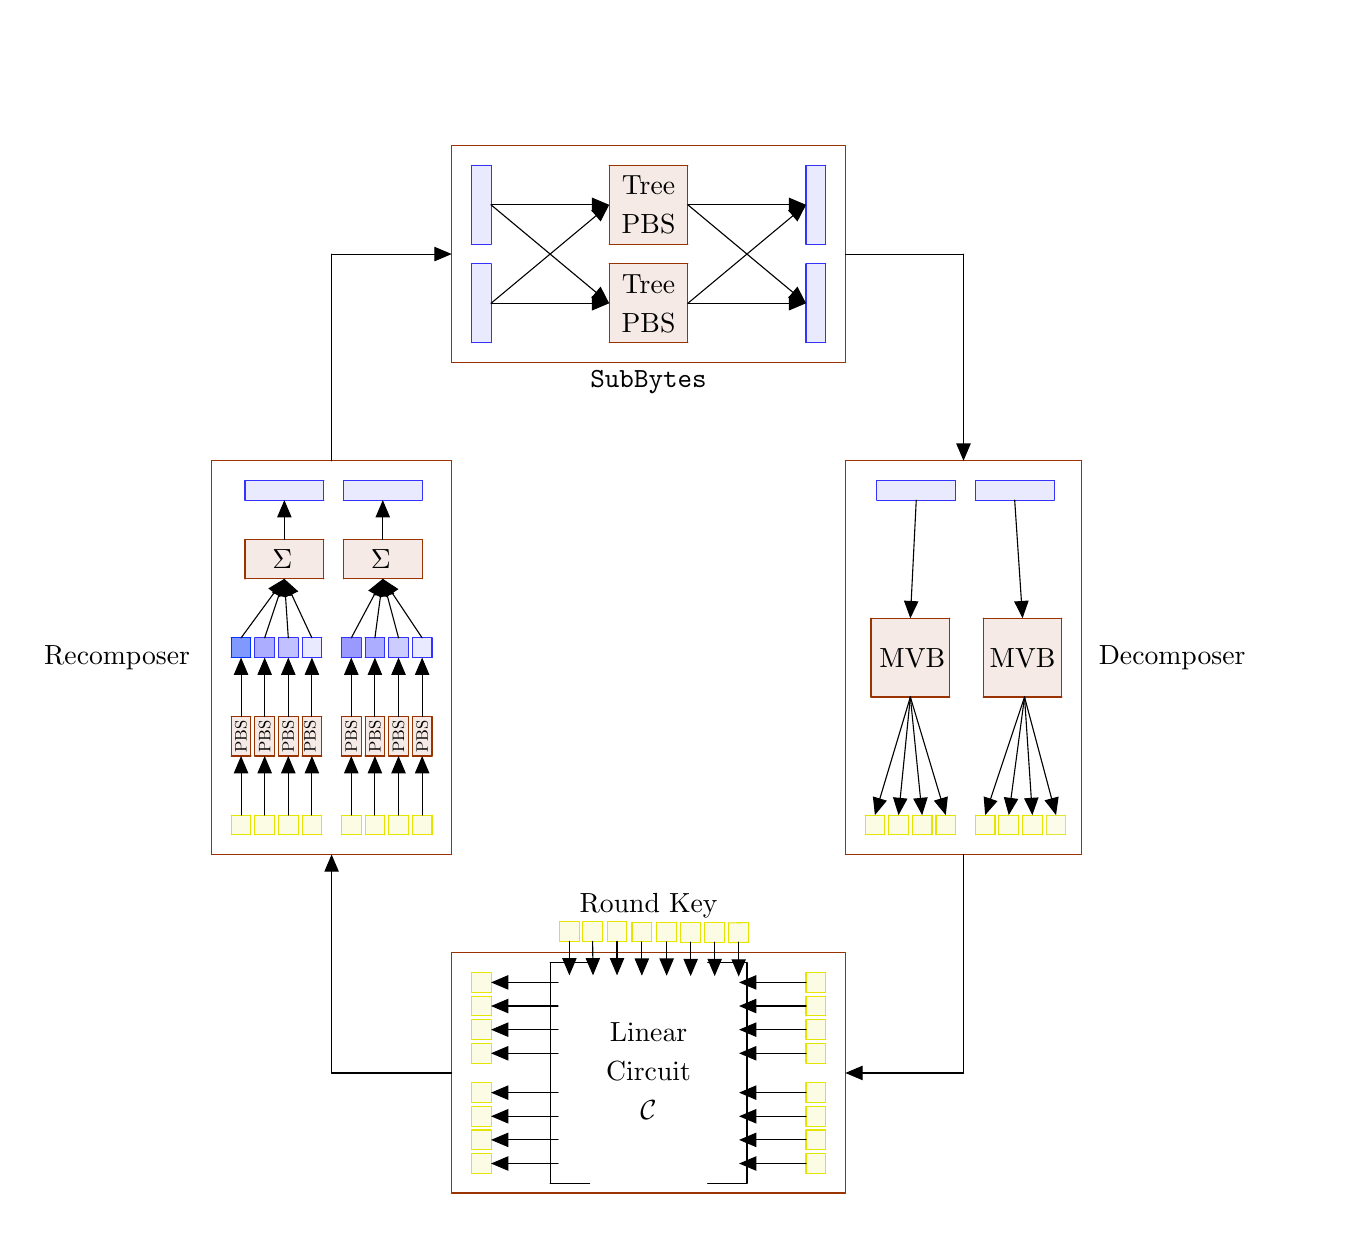
\begin{tikzpicture}[line cap=round,line join=round,>=triangle 45,x=0.5cm,y=0.5cm]
\clip(-10.77,-27) rectangle (22,3);
\fill[color=ttttff,fill=ttttff,fill opacity=0.1] (0.5,-0.5) -- (1,-0.5) -- (1,-2.5) -- (0.5,-2.5) -- cycle;
\fill[color=ttttff,fill=ttttff,fill opacity=0.1] (0.5,-3) -- (1,-3) -- (1,-5) -- (0.5,-5) -- cycle;
\fill[color=zzttqq,fill=zzttqq,fill opacity=0.1] (4,-0.5) -- (6,-0.5) -- (6,-2.5) -- (4,-2.5) -- cycle;
\fill[color=zzttqq,fill=zzttqq,fill opacity=0.1] (4,-3) -- (6,-3) -- (6,-5) -- (4,-5) -- cycle;
\fill[color=ttttff,fill=ttttff,fill opacity=0.1] (9,-0.5) -- (9.5,-0.5) -- (9.5,-2.5) -- (9,-2.5) -- cycle;
\fill[color=ttttff,fill=ttttff,fill opacity=0.1] (9,-3) -- (9.5,-3) -- (9.5,-5) -- (9,-5) -- cycle;
\fill[color=ttttff,fill=ttttff,fill opacity=0.1] (10.8,-8.5) -- (12.8,-8.5) -- (12.8,-9) -- (10.8,-9) -- cycle;
\fill[color=ttttff,fill=ttttff,fill opacity=0.1] (13.3,-8.5) -- (15.3,-8.5) -- (15.3,-9) -- (13.3,-9) -- cycle;
\fill[color=ffffqq,fill=ffffqq,fill opacity=0.1] (10.5,-17) -- (11,-17) -- (11,-17.5) -- (10.5,-17.5) -- cycle;
\fill[color=ffffqq,fill=ffffqq,fill opacity=0.1] (11.1,-17) -- (11.6,-17) -- (11.6,-17.5) -- (11.1,-17.5) -- cycle;
\fill[color=ffffqq,fill=ffffqq,fill opacity=0.1] (11.7,-17) -- (12.2,-17) -- (12.2,-17.5) -- (11.7,-17.5) -- cycle;
\fill[color=ffffqq,fill=ffffqq,fill opacity=0.1] (12.3,-17) -- (12.8,-17) -- (12.8,-17.5) -- (12.3,-17.5) -- cycle;
\fill[color=ffffqq,fill=ffffqq,fill opacity=0.1] (13.3,-17) -- (13.8,-17) -- (13.8,-17.5) -- (13.3,-17.5) -- cycle;
\fill[color=ffffqq,fill=ffffqq,fill opacity=0.1] (13.9,-17) -- (14.4,-17) -- (14.4,-17.5) -- (13.9,-17.5) -- cycle;
\fill[color=ffffqq,fill=ffffqq,fill opacity=0.1] (14.5,-17) -- (15,-17) -- (15,-17.5) -- (14.5,-17.5) -- cycle;
\fill[color=fffftt,fill=fffftt,fill opacity=0.1] (15.1,-17) -- (15.6,-17) -- (15.6,-17.5) -- (15.1,-17.5) -- cycle;
\fill[color=zzttqq,fill=zzttqq,fill opacity=0.1] (10.65,-12) -- (12.65,-12) -- (12.65,-14) -- (10.65,-14) -- cycle;
\fill[color=zzttqq,fill=zzttqq,fill opacity=0.1] (13.5,-12) -- (15.5,-12) -- (15.5,-14) -- (13.5,-14) -- cycle;
\fill[color=ffffqq,fill=ffffqq,fill opacity=0.1] (-5.6,-17) -- (-5.1,-17) -- (-5.1,-17.5) -- (-5.6,-17.5) -- cycle;
\fill[color=ffffqq,fill=ffffqq,fill opacity=0.1] (-5,-17) -- (-4.5,-17) -- (-4.5,-17.5) -- (-5,-17.5) -- cycle;
\fill[color=ffffqq,fill=ffffqq,fill opacity=0.1] (-4.4,-17) -- (-3.9,-17) -- (-3.9,-17.5) -- (-4.4,-17.5) -- cycle;
\fill[color=ffffqq,fill=ffffqq,fill opacity=0.1] (-3.8,-17) -- (-3.3,-17) -- (-3.3,-17.5) -- (-3.8,-17.5) -- cycle;
\fill[color=ffffqq,fill=ffffqq,fill opacity=0.1] (-2.8,-17) -- (-2.3,-17) -- (-2.3,-17.5) -- (-2.8,-17.5) -- cycle;
\fill[color=ffffqq,fill=ffffqq,fill opacity=0.1] (-2.2,-17) -- (-1.7,-17) -- (-1.7,-17.5) -- (-2.2,-17.5) -- cycle;
\fill[color=ffffqq,fill=ffffqq,fill opacity=0.1] (-1.6,-17) -- (-1.1,-17) -- (-1.1,-17.5) -- (-1.6,-17.5) -- cycle;
\fill[color=ffffqq,fill=ffffqq,fill opacity=0.1] (-1,-17) -- (-0.5,-17) -- (-0.5,-17.5) -- (-1,-17.5) -- cycle;
\fill[color=zzttqq,fill=zzttqq,fill opacity=0.1] (-5.6,-14.5) -- (-5.1,-14.5) -- (-5.1,-15.5) -- (-5.6,-15.5) -- cycle;
\fill[color=zzttqq,fill=zzttqq,fill opacity=0.1] (-5,-14.5) -- (-4.5,-14.5) -- (-4.5,-15.5) -- (-5,-15.5) -- cycle;
\fill[color=zzttqq,fill=zzttqq,fill opacity=0.1] (-4.4,-14.5) -- (-3.9,-14.5) -- (-3.9,-15.5) -- (-4.4,-15.5) -- cycle;
\fill[color=zzttqq,fill=zzttqq,fill opacity=0.1] (-3.8,-14.5) -- (-3.3,-14.5) -- (-3.3,-15.5) -- (-3.8,-15.5) -- cycle;
\fill[color=zzttqq,fill=zzttqq,fill opacity=0.1] (-2.8,-14.5) -- (-2.3,-14.5) -- (-2.3,-15.5) -- (-2.8,-15.5) -- cycle;
\fill[color=zzttqq,fill=zzttqq,fill opacity=0.1] (-2.2,-14.5) -- (-1.7,-14.5) -- (-1.7,-15.5) -- (-2.2,-15.5) -- cycle;
\fill[color=zzttqq,fill=zzttqq,fill opacity=0.1] (-1.6,-14.5) -- (-1.1,-14.5) -- (-1.1,-15.5) -- (-1.6,-15.5) -- cycle;
\fill[color=zzttqq,fill=zzttqq,fill opacity=0.1] (-1,-14.5) -- (-0.5,-14.5) -- (-0.5,-15.5) -- (-1,-15.5) -- cycle;
\fill[color=qqttff,fill=qqttff,fill opacity=0.5] (-5.6,-12.5) -- (-5.1,-12.5) -- (-5.1,-13) -- (-5.6,-13) -- cycle;
\fill[color=ttttff,fill=ttttff,fill opacity=0.3] (-4.4,-12.5) -- (-3.9,-12.5) -- (-3.9,-13) -- (-4.4,-13) -- cycle;
\fill[color=ttttff,fill=ttttff,fill opacity=0.4] (-5,-12.5) -- (-4.5,-12.5) -- (-4.5,-13) -- (-5,-13) -- cycle;
\fill[color=ttttff,fill=ttttff,fill opacity=0.1] (-3.8,-12.5) -- (-3.3,-12.5) -- (-3.3,-13) -- (-3.8,-13) -- cycle;
\fill[color=ttttff,fill=ttttff,fill opacity=0.5] (-2.8,-12.5) -- (-2.3,-12.5) -- (-2.3,-13) -- (-2.8,-13) -- cycle;
\fill[color=ttttff,fill=ttttff,fill opacity=0.4] (-2.2,-12.5) -- (-1.7,-12.5) -- (-1.7,-13) -- (-2.2,-13) -- cycle;
\fill[color=ttttff,fill=ttttff,fill opacity=0.25] (-1.6,-12.5) -- (-1.1,-12.5) -- (-1.1,-13) -- (-1.6,-13) -- cycle;
\fill[color=ttttff,fill=ttttff,fill opacity=0.1] (-1,-12.5) -- (-0.5,-12.5) -- (-0.5,-13) -- (-1,-13) -- cycle;
\fill[color=zzttqq,fill=zzttqq,fill opacity=0.1] (-5.25,-10) -- (-3.25,-10) -- (-3.25,-11) -- (-5.25,-11) -- cycle;
\fill[color=zzttqq,fill=zzttqq,fill opacity=0.1] (-2.75,-10) -- (-0.75,-10) -- (-0.75,-11) -- (-2.75,-11) -- cycle;
\fill[color=ttttff,fill=ttttff,fill opacity=0.1] (-5.25,-8.5) -- (-3.25,-8.5) -- (-3.25,-9) -- (-5.25,-9) -- cycle;
\fill[color=ttttff,fill=ttttff,fill opacity=0.1] (-2.75,-8.5) -- (-0.75,-8.5) -- (-0.75,-9) -- (-2.75,-9) -- cycle;
\fill[color=ffffqq,fill=ffffqq,fill opacity=0.1] (0.5,-21) -- (1,-21) -- (1,-21.5) -- (0.5,-21.5) -- cycle;
\fill[color=ffffqq,fill=ffffqq,fill opacity=0.1] (0.5,-21.6) -- (1,-21.6) -- (1,-22.1) -- (0.5,-22.1) -- cycle;
\fill[color=ffffqq,fill=ffffqq,fill opacity=0.1] (0.5,-22.2) -- (1,-22.2) -- (1,-22.7) -- (0.5,-22.7) -- cycle;
\fill[color=ffffqq,fill=ffffqq,fill opacity=0.1] (0.5,-22.8) -- (1,-22.8) -- (1,-23.3) -- (0.5,-23.3) -- cycle;
\fill[color=ffffqq,fill=ffffqq,fill opacity=0.1] (0.5,-23.8) -- (1,-23.8) -- (1,-24.3) -- (0.5,-24.3) -- cycle;
\fill[color=ffffqq,fill=ffffqq,fill opacity=0.1] (0.5,-24.4) -- (1,-24.4) -- (1,-24.9) -- (0.5,-24.9) -- cycle;
\fill[color=ffffqq,fill=ffffqq,fill opacity=0.1] (0.5,-25) -- (1,-25) -- (1,-25.5) -- (0.5,-25.5) -- cycle;
\fill[color=ffffqq,fill=ffffqq,fill opacity=0.1] (0.5,-25.6) -- (1,-25.6) -- (1,-26.1) -- (0.5,-26.1) -- cycle;
\fill[color=ffffqq,fill=ffffqq,fill opacity=0.1] (9,-23.8) -- (9.5,-23.8) -- (9.5,-24.3) -- (9,-24.3) -- cycle;
\fill[color=ffffqq,fill=ffffqq,fill opacity=0.1] (9,-24.4) -- (9.5,-24.4) -- (9.5,-24.9) -- (9,-24.9) -- cycle;
\fill[color=ffffqq,fill=ffffqq,fill opacity=0.1] (9,-25) -- (9.5,-25) -- (9.5,-25.5) -- (9,-25.5) -- cycle;
\fill[color=ffffqq,fill=ffffqq,fill opacity=0.1] (9,-25.6) -- (9.5,-25.6) -- (9.5,-26.1) -- (9,-26.1) -- cycle;
\fill[color=ffffqq,fill=ffffqq,fill opacity=0.1] (9,-23.3) -- (9.5,-23.3) -- (9.5,-22.8) -- (9,-22.8) -- cycle;
\fill[color=ffffqq,fill=ffffqq,fill opacity=0.1] (9,-22.7) -- (9.5,-22.7) -- (9.5,-22.2) -- (9,-22.2) -- cycle;
\fill[color=ffffqq,fill=ffffqq,fill opacity=0.1] (9,-22.1) -- (9.5,-22.1) -- (9.5,-21.6) -- (9,-21.6) -- cycle;
\fill[color=ffffqq,fill=ffffqq,fill opacity=0.1] (9,-21.5) -- (9.5,-21.5) -- (9.5,-21) -- (9,-21) -- cycle;
\fill[color=ffffqq,fill=ffffqq,fill opacity=0.1] (2.74,-19.71) -- (3.24,-19.71) -- (3.24,-20.21) -- (2.74,-20.21) -- cycle;
\fill[color=ffffqq,fill=ffffqq,fill opacity=0.1] (3.33,-19.71) -- (3.83,-19.71) -- (3.83,-20.21) -- (3.33,-20.21) -- cycle;
\fill[color=ffffqq,fill=ffffqq,fill opacity=0.1] (3.95,-19.71) -- (4.45,-19.71) -- (4.45,-20.21) -- (3.95,-20.21) -- cycle;
\fill[color=ffffqq,fill=ffffqq,fill opacity=0.1] (4.58,-19.72) -- (5.08,-19.72) -- (5.08,-20.22) -- (4.58,-20.22) -- cycle;
\fill[color=ffffqq,fill=ffffqq,fill opacity=0.1] (5.21,-19.72) -- (5.71,-19.72) -- (5.71,-20.22) -- (5.21,-20.22) -- cycle;
\fill[color=ffffqq,fill=ffffqq,fill opacity=0.1] (5.82,-19.73) -- (6.32,-19.73) -- (6.32,-20.23) -- (5.82,-20.23) -- cycle;
\fill[color=ffffqq,fill=ffffqq,fill opacity=0.1] (6.43,-19.73) -- (6.93,-19.73) -- (6.93,-20.23) -- (6.43,-20.23) -- cycle;
\fill[color=ffffqq,fill=ffffqq,fill opacity=0.1] (7.02,-19.74) -- (7.55,-19.73) -- (7.55,-20.23) -- (7.02,-20.24) -- cycle;
\draw [color=zzttqq] (0,0)-- (10,0);
\draw [color=zzttqq] (10,0)-- (10,-5.5);
\draw [color=zzttqq] (10,-5.5)-- (0,-5.5);
\draw [color=zzttqq] (0,-5.5)-- (0,0);
\draw [color=ttttff] (0.5,-0.5)-- (1,-0.5);
\draw [color=ttttff] (1,-0.5)-- (1,-2.5);
\draw [color=ttttff] (1,-2.5)-- (0.5,-2.5);
\draw [color=ttttff] (0.5,-2.5)-- (0.5,-0.5);
\draw [color=ttttff] (0.5,-3)-- (1,-3);
\draw [color=ttttff] (1,-3)-- (1,-5);
\draw [color=ttttff] (1,-5)-- (0.5,-5);
\draw [color=ttttff] (0.5,-5)-- (0.5,-3);
\draw [color=zzttqq] (4,-0.5)-- (6,-0.5);
\draw [color=zzttqq] (6,-0.5)-- (6,-2.5);
\draw [color=zzttqq] (6,-2.5)-- (4,-2.5);
\draw [color=zzttqq] (4,-2.5)-- (4,-0.5);
\draw [color=zzttqq] (4,-3)-- (6,-3);
\draw [color=zzttqq] (6,-3)-- (6,-5);
\draw [color=zzttqq] (6,-5)-- (4,-5);
\draw [color=zzttqq] (4,-5)-- (4,-3);
\draw [color=ttttff] (9,-0.5)-- (9.5,-0.5);
\draw [color=ttttff] (9.5,-0.5)-- (9.5,-2.5);
\draw [color=ttttff] (9.5,-2.5)-- (9,-2.5);
\draw [color=ttttff] (9,-2.5)-- (9,-0.5);
\draw [color=ttttff] (9,-3)-- (9.5,-3);
\draw [color=ttttff] (9.5,-3)-- (9.5,-5);
\draw [color=ttttff] (9.5,-5)-- (9,-5);
\draw [color=ttttff] (9,-5)-- (9,-3);
\draw [->] (1,-1.5) -- (4,-1.5);
\draw [->] (1,-4) -- (4,-4);
\draw [->] (1,-4) -- (4,-1.5);
\draw [->] (1,-1.5) -- (4,-4);
\draw [->] (6,-1.5) -- (9,-1.5);
\draw [->] (6,-1.5) -- (9,-4);
\draw [->] (6,-4) -- (9,-4);
\draw [->] (6,-4) -- (9,-1.5);
\draw [color=zzttqq] (10,-8)-- (16,-8);
\draw [color=zzttqq] (16,-8)-- (16,-18);
\draw [color=zzttqq] (16,-18)-- (10,-18);
\draw [color=zzttqq] (10,-18)-- (10,-8);
\draw [color=ttttff] (10.8,-8.5)-- (12.8,-8.5);
\draw [color=ttttff] (12.8,-8.5)-- (12.8,-9);
\draw [color=ttttff] (12.8,-9)-- (10.8,-9);
\draw [color=ttttff] (10.8,-9)-- (10.8,-8.5);
\draw [color=ttttff] (13.3,-8.5)-- (15.3,-8.5);
\draw [color=ttttff] (15.3,-8.5)-- (15.3,-9);
\draw [color=ttttff] (15.3,-9)-- (13.3,-9);
\draw [color=ttttff] (13.3,-9)-- (13.3,-8.5);
\draw [color=ffffqq] (10.5,-17)-- (11,-17);
\draw [color=ffffqq] (11,-17)-- (11,-17.5);
\draw [color=ffffqq] (11,-17.5)-- (10.5,-17.5);
\draw [color=ffffqq] (10.5,-17.5)-- (10.5,-17);
\draw [color=ffffqq] (11.1,-17)-- (11.6,-17);
\draw [color=ffffqq] (11.6,-17)-- (11.6,-17.5);
\draw [color=ffffqq] (11.6,-17.5)-- (11.1,-17.5);
\draw [color=ffffqq] (11.1,-17.5)-- (11.1,-17);
\draw [color=ffffqq] (11.7,-17)-- (12.2,-17);
\draw [color=ffffqq] (12.2,-17)-- (12.2,-17.5);
\draw [color=ffffqq] (12.2,-17.5)-- (11.7,-17.5);
\draw [color=ffffqq] (11.7,-17.5)-- (11.7,-17);
\draw [color=ffffqq] (12.3,-17)-- (12.8,-17);
\draw [color=ffffqq] (12.8,-17)-- (12.8,-17.5);
\draw [color=ffffqq] (12.8,-17.5)-- (12.3,-17.5);
\draw [color=ffffqq] (12.3,-17.5)-- (12.3,-17);
\draw [color=ffffqq] (13.3,-17)-- (13.8,-17);
\draw [color=ffffqq] (13.8,-17)-- (13.8,-17.5);
\draw [color=ffffqq] (13.8,-17.5)-- (13.3,-17.5);
\draw [color=ffffqq] (13.3,-17.5)-- (13.3,-17);
\draw [color=ffffqq] (13.9,-17)-- (14.4,-17);
\draw [color=ffffqq] (14.4,-17)-- (14.4,-17.5);
\draw [color=ffffqq] (14.4,-17.5)-- (13.9,-17.5);
\draw [color=ffffqq] (13.9,-17.5)-- (13.9,-17);
\draw [color=ffffqq] (14.5,-17)-- (15,-17);
\draw [color=ffffqq] (15,-17)-- (15,-17.5);
\draw [color=ffffqq] (15,-17.5)-- (14.5,-17.5);
\draw [color=ffffqq] (14.5,-17.5)-- (14.5,-17);
\draw [color=fffftt] (15.1,-17)-- (15.6,-17);
\draw [color=fffftt] (15.6,-17)-- (15.6,-17.5);
\draw [color=fffftt] (15.6,-17.5)-- (15.1,-17.5);
\draw [color=fffftt] (15.1,-17.5)-- (15.1,-17);
\draw [color=zzttqq] (10.65,-12)-- (12.65,-12);
\draw [color=zzttqq] (12.65,-12)-- (12.65,-14);
\draw [color=zzttqq] (12.65,-14)-- (10.65,-14);
\draw [color=zzttqq] (10.65,-14)-- (10.65,-12);
\draw [color=zzttqq] (13.5,-12)-- (15.5,-12);
\draw [color=zzttqq] (15.5,-12)-- (15.5,-14);
\draw [color=zzttqq] (15.5,-14)-- (13.5,-14);
\draw [color=zzttqq] (13.5,-14)-- (13.5,-12);
\draw [->] (11.8,-9) -- (11.65,-12);
\draw [->] (14.3,-9) -- (14.5,-12);
\draw [->] (11.65,-14) -- (10.75,-17);
\draw [->] (11.65,-14) -- (11.35,-17);
\draw [->] (11.65,-14) -- (11.95,-17);
\draw [->] (11.65,-14) -- (12.55,-17);
\draw [->] (14.55,-14) -- (13.55,-17);
\draw [->] (14.55,-14) -- (14.15,-17);
\draw [->] (14.55,-14) -- (14.75,-17);
\draw [->] (14.55,-14) -- (15.35,-17);
\draw [color=zzttqq] (-6.1,-8)-- (0,-8);
\draw [color=zzttqq] (0,-8)-- (0,-18);
\draw [color=zzttqq] (0,-18)-- (-6.1,-18);
\draw [color=zzttqq] (-6.1,-18)-- (-6.1,-8);
\draw [color=ffffqq] (-5.6,-17)-- (-5.1,-17);
\draw [color=ffffqq] (-5.1,-17)-- (-5.1,-17.5);
\draw [color=ffffqq] (-5.1,-17.5)-- (-5.6,-17.5);
\draw [color=ffffqq] (-5.6,-17.5)-- (-5.6,-17);
\draw [color=ffffqq] (-5,-17)-- (-4.5,-17);
\draw [color=ffffqq] (-4.5,-17)-- (-4.5,-17.5);
\draw [color=ffffqq] (-4.5,-17.5)-- (-5,-17.5);
\draw [color=ffffqq] (-5,-17.5)-- (-5,-17);
\draw [color=ffffqq] (-4.4,-17)-- (-3.9,-17);
\draw [color=ffffqq] (-3.9,-17)-- (-3.9,-17.5);
\draw [color=ffffqq] (-3.9,-17.5)-- (-4.4,-17.5);
\draw [color=ffffqq] (-4.4,-17.5)-- (-4.4,-17);
\draw [color=ffffqq] (-3.8,-17)-- (-3.3,-17);
\draw [color=ffffqq] (-3.3,-17)-- (-3.3,-17.5);
\draw [color=ffffqq] (-3.3,-17.5)-- (-3.8,-17.5);
\draw [color=ffffqq] (-3.8,-17.5)-- (-3.8,-17);
\draw [color=ffffqq] (-2.8,-17)-- (-2.3,-17);
\draw [color=ffffqq] (-2.3,-17)-- (-2.3,-17.5);
\draw [color=ffffqq] (-2.3,-17.5)-- (-2.8,-17.5);
\draw [color=ffffqq] (-2.8,-17.5)-- (-2.8,-17);
\draw [color=ffffqq] (-2.2,-17)-- (-1.7,-17);
\draw [color=ffffqq] (-1.7,-17)-- (-1.7,-17.5);
\draw [color=ffffqq] (-1.7,-17.5)-- (-2.2,-17.5);
\draw [color=ffffqq] (-2.2,-17.5)-- (-2.2,-17);
\draw [color=ffffqq] (-1.6,-17)-- (-1.1,-17);
\draw [color=ffffqq] (-1.1,-17)-- (-1.1,-17.5);
\draw [color=ffffqq] (-1.1,-17.5)-- (-1.6,-17.5);
\draw [color=ffffqq] (-1.6,-17.5)-- (-1.6,-17);
\draw [color=ffffqq] (-1,-17)-- (-0.5,-17);
\draw [color=ffffqq] (-0.5,-17)-- (-0.5,-17.5);
\draw [color=ffffqq] (-0.5,-17.5)-- (-1,-17.5);
\draw [color=ffffqq] (-1,-17.5)-- (-1,-17);
\draw [color=zzttqq] (-5.6,-14.5)-- (-5.1,-14.5);
\draw [color=zzttqq] (-5.1,-14.5)-- (-5.1,-15.5);
\draw [color=zzttqq] (-5.1,-15.5)-- (-5.6,-15.5);
\draw [color=zzttqq] (-5.6,-15.5)-- (-5.6,-14.5);
\draw [color=zzttqq] (-5,-14.5)-- (-4.5,-14.5);
\draw [color=zzttqq] (-4.5,-14.5)-- (-4.5,-15.5);
\draw [color=zzttqq] (-4.5,-15.5)-- (-5,-15.5);
\draw [color=zzttqq] (-5,-15.5)-- (-5,-14.5);
\draw [color=zzttqq] (-4.4,-14.5)-- (-3.9,-14.5);
\draw [color=zzttqq] (-3.9,-14.5)-- (-3.9,-15.5);
\draw [color=zzttqq] (-3.9,-15.5)-- (-4.4,-15.5);
\draw [color=zzttqq] (-4.4,-15.5)-- (-4.4,-14.5);
\draw [color=zzttqq] (-3.8,-14.5)-- (-3.3,-14.5);
\draw [color=zzttqq] (-3.3,-14.5)-- (-3.3,-15.5);
\draw [color=zzttqq] (-3.3,-15.5)-- (-3.8,-15.5);
\draw [color=zzttqq] (-3.8,-15.5)-- (-3.8,-14.5);
\draw [color=zzttqq] (-2.8,-14.5)-- (-2.3,-14.5);
\draw [color=zzttqq] (-2.3,-14.5)-- (-2.3,-15.5);
\draw [color=zzttqq] (-2.3,-15.5)-- (-2.8,-15.5);
\draw [color=zzttqq] (-2.8,-15.5)-- (-2.8,-14.5);
\draw [color=zzttqq] (-2.2,-14.5)-- (-1.7,-14.5);
\draw [color=zzttqq] (-1.7,-14.5)-- (-1.7,-15.5);
\draw [color=zzttqq] (-1.7,-15.5)-- (-2.2,-15.5);
\draw [color=zzttqq] (-2.2,-15.5)-- (-2.2,-14.5);
\draw [color=zzttqq] (-1.6,-14.5)-- (-1.1,-14.5);
\draw [color=zzttqq] (-1.1,-14.5)-- (-1.1,-15.5);
\draw [color=zzttqq] (-1.1,-15.5)-- (-1.6,-15.5);
\draw [color=zzttqq] (-1.6,-15.5)-- (-1.6,-14.5);
\draw [->] (-5.35,-17) -- (-5.35,-15.5);
\draw [->] (-4.75,-17) -- (-4.75,-15.5);
\draw [->] (-4.15,-17) -- (-4.15,-15.5);
\draw [->] (-3.55,-17) -- (-3.55,-15.5);
\draw [color=zzttqq] (-1,-14.5)-- (-0.5,-14.5);
\draw [color=zzttqq] (-0.5,-14.5)-- (-0.5,-15.5);
\draw [color=zzttqq] (-0.5,-15.5)-- (-1,-15.5);
\draw [color=zzttqq] (-1,-15.5)-- (-1,-14.5);
\draw [->] (-2.55,-17) -- (-2.55,-15.5);
\draw [->] (-1.95,-17) -- (-1.95,-15.5);
\draw [->] (-1.35,-17) -- (-1.35,-15.5);
\draw [->] (-0.75,-17) -- (-0.75,-15.5);
\draw [color=qqttff] (-5.6,-12.5)-- (-5.1,-12.5);
\draw [color=qqttff] (-5.1,-12.5)-- (-5.1,-13);
\draw [color=qqttff] (-5.1,-13)-- (-5.6,-13);
\draw [color=qqttff] (-5.6,-13)-- (-5.6,-12.5);
\draw [color=ttttff] (-4.4,-12.5)-- (-3.9,-12.5);
\draw [color=ttttff] (-3.9,-12.5)-- (-3.9,-13);
\draw [color=ttttff] (-3.9,-13)-- (-4.4,-13);
\draw [color=ttttff] (-4.4,-13)-- (-4.4,-12.5);
\draw [color=ttttff] (-5,-12.5)-- (-4.5,-12.5);
\draw [color=ttttff] (-4.5,-12.5)-- (-4.5,-13);
\draw [color=ttttff] (-4.5,-13)-- (-5,-13);
\draw [color=ttttff] (-5,-13)-- (-5,-12.5);
\draw [color=ttttff] (-3.8,-12.5)-- (-3.3,-12.5);
\draw [color=ttttff] (-3.3,-12.5)-- (-3.3,-13);
\draw [color=ttttff] (-3.3,-13)-- (-3.8,-13);
\draw [color=ttttff] (-3.8,-13)-- (-3.8,-12.5);
\draw [color=ttttff] (-2.8,-12.5)-- (-2.3,-12.5);
\draw [color=ttttff] (-2.3,-12.5)-- (-2.3,-13);
\draw [color=ttttff] (-2.3,-13)-- (-2.8,-13);
\draw [color=ttttff] (-2.8,-13)-- (-2.8,-12.5);
\draw [color=ttttff] (-2.2,-12.5)-- (-1.7,-12.5);
\draw [color=ttttff] (-1.7,-12.5)-- (-1.7,-13);
\draw [color=ttttff] (-1.7,-13)-- (-2.2,-13);
\draw [color=ttttff] (-2.2,-13)-- (-2.2,-12.5);
\draw [color=ttttff] (-1.6,-12.5)-- (-1.1,-12.5);
\draw [color=ttttff] (-1.1,-12.5)-- (-1.1,-13);
\draw [color=ttttff] (-1.1,-13)-- (-1.6,-13);
\draw [color=ttttff] (-1.6,-13)-- (-1.6,-12.5);
\draw [color=ttttff] (-1,-12.5)-- (-0.5,-12.5);
\draw [color=ttttff] (-0.5,-12.5)-- (-0.5,-13);
\draw [color=ttttff] (-0.5,-13)-- (-1,-13);
\draw [color=ttttff] (-1,-13)-- (-1,-12.5);
\draw [->] (-5.35,-14.5) -- (-5.35,-13);
\draw [->] (-4.75,-14.5) -- (-4.75,-13);
\draw [->] (-4.15,-14.5) -- (-4.15,-13);
\draw [->] (-3.55,-14.5) -- (-3.55,-13);
\draw [->] (-2.55,-14.5) -- (-2.55,-13);
\draw [->] (-1.95,-14.5) -- (-1.95,-13);
\draw [->] (-1.35,-14.5) -- (-1.35,-13);
\draw [->] (-0.75,-14.5) -- (-0.75,-13);
\draw [color=zzttqq] (-5.25,-10)-- (-3.25,-10);
\draw [color=zzttqq] (-3.25,-10)-- (-3.25,-11);
\draw [color=zzttqq] (-3.25,-11)-- (-5.25,-11);
\draw [color=zzttqq] (-5.25,-11)-- (-5.25,-10);
\draw [color=zzttqq] (-2.75,-10)-- (-0.75,-10);
\draw [color=zzttqq] (-0.75,-10)-- (-0.75,-11);
\draw [color=zzttqq] (-0.75,-11)-- (-2.75,-11);
\draw [color=zzttqq] (-2.75,-11)-- (-2.75,-10);
\draw [->] (-5.35,-12.5) -- (-4.25,-11);
\draw [->] (-4.75,-12.5) -- (-4.25,-11);
\draw [->] (-4.15,-12.5) -- (-4.25,-11);
\draw [->] (-3.55,-12.5) -- (-4.25,-11);
\draw [->] (-2.55,-12.5) -- (-1.75,-11);
\draw [->] (-1.95,-12.5) -- (-1.75,-11);
\draw [->] (-1.35,-12.5) -- (-1.75,-11);
\draw [->] (-0.75,-12.5) -- (-1.75,-11);
\draw [color=ttttff] (-5.25,-8.5)-- (-3.25,-8.5);
\draw [color=ttttff] (-3.25,-8.5)-- (-3.25,-9);
\draw [color=ttttff] (-3.25,-9)-- (-5.25,-9);
\draw [color=ttttff] (-5.25,-9)-- (-5.25,-8.5);
\draw [color=ttttff] (-2.75,-8.5)-- (-0.75,-8.5);
\draw [color=ttttff] (-0.75,-8.5)-- (-0.75,-9);
\draw [color=ttttff] (-0.75,-9)-- (-2.75,-9);
\draw [color=ttttff] (-2.75,-9)-- (-2.75,-8.5);
\draw [->] (-4.25,-10) -- (-4.25,-9);
\draw [->] (-1.75,-10) -- (-1.75,-9);
\draw [color=ffffqq] (0.5,-21)-- (1,-21);
\draw [color=ffffqq] (1,-21)-- (1,-21.5);
\draw [color=ffffqq] (1,-21.5)-- (0.5,-21.5);
\draw [color=ffffqq] (0.5,-21.5)-- (0.5,-21);
\draw [color=ffffqq] (0.5,-21.6)-- (1,-21.6);
\draw [color=ffffqq] (1,-21.6)-- (1,-22.1);
\draw [color=ffffqq] (1,-22.1)-- (0.5,-22.1);
\draw [color=ffffqq] (0.5,-22.1)-- (0.5,-21.6);
\draw [color=ffffqq] (0.5,-22.2)-- (1,-22.2);
\draw [color=ffffqq] (1,-22.2)-- (1,-22.7);
\draw [color=ffffqq] (1,-22.7)-- (0.5,-22.7);
\draw [color=ffffqq] (0.5,-22.7)-- (0.5,-22.2);
\draw [color=ffffqq] (0.5,-22.8)-- (1,-22.8);
\draw [color=ffffqq] (1,-22.8)-- (1,-23.3);
\draw [color=ffffqq] (1,-23.3)-- (0.5,-23.3);
\draw [color=ffffqq] (0.5,-23.3)-- (0.5,-22.8);
\draw [color=ffffqq] (0.5,-23.8)-- (1,-23.8);
\draw [color=ffffqq] (1,-23.8)-- (1,-24.3);
\draw [color=ffffqq] (1,-24.3)-- (0.5,-24.3);
\draw [color=ffffqq] (0.5,-24.3)-- (0.5,-23.8);
\draw [color=ffffqq] (0.5,-24.4)-- (1,-24.4);
\draw [color=ffffqq] (1,-24.4)-- (1,-24.9);
\draw [color=ffffqq] (1,-24.9)-- (0.5,-24.9);
\draw [color=ffffqq] (0.5,-24.9)-- (0.5,-24.4);
\draw [color=ffffqq] (0.5,-25)-- (1,-25);
\draw [color=ffffqq] (1,-25)-- (1,-25.5);
\draw [color=ffffqq] (1,-25.5)-- (0.5,-25.5);
\draw [color=ffffqq] (0.5,-25.5)-- (0.5,-25);
\draw [color=ffffqq] (0.5,-25.6)-- (1,-25.6);
\draw [color=ffffqq] (1,-25.6)-- (1,-26.1);
\draw [color=ffffqq] (1,-26.1)-- (0.5,-26.1);
\draw [color=ffffqq] (0.5,-26.1)-- (0.5,-25.6);
\draw [color=zzttqq] (0,-20.5)-- (10,-20.5);
\draw [color=zzttqq] (10,-20.5)-- (10,-26.6);
\draw [color=zzttqq] (10,-26.6)-- (0,-26.6);
\draw [color=zzttqq] (0,-26.6)-- (0,-20.5);
\draw [color=ffffqq] (9,-23.8)-- (9.5,-23.8);
\draw [color=ffffqq] (9.5,-23.8)-- (9.5,-24.3);
\draw [color=ffffqq] (9.5,-24.3)-- (9,-24.3);
\draw [color=ffffqq] (9,-24.3)-- (9,-23.8);
\draw [color=ffffqq] (9,-24.4)-- (9.5,-24.4);
\draw [color=ffffqq] (9.5,-24.4)-- (9.5,-24.9);
\draw [color=ffffqq] (9.5,-24.9)-- (9,-24.9);
\draw [color=ffffqq] (9,-24.9)-- (9,-24.4);
\draw [color=ffffqq] (9,-25)-- (9.5,-25);
\draw [color=ffffqq] (9.5,-25)-- (9.5,-25.5);
\draw [color=ffffqq] (9.5,-25.5)-- (9,-25.5);
\draw [color=ffffqq] (9,-25.5)-- (9,-25);
\draw [color=ffffqq] (9,-25.6)-- (9.5,-25.6);
\draw [color=ffffqq] (9.5,-25.6)-- (9.5,-26.1);
\draw [color=ffffqq] (9.5,-26.1)-- (9,-26.1);
\draw [color=ffffqq] (9,-26.1)-- (9,-25.6);
\draw [color=ffffqq] (9,-23.3)-- (9.5,-23.3);
\draw [color=ffffqq] (9.5,-23.3)-- (9.5,-22.8);
\draw [color=ffffqq] (9.5,-22.8)-- (9,-22.8);
\draw [color=ffffqq] (9,-22.8)-- (9,-23.3);
\draw [color=ffffqq] (9,-22.7)-- (9.5,-22.7);
\draw [color=ffffqq] (9.5,-22.7)-- (9.5,-22.2);
\draw [color=ffffqq] (9.5,-22.2)-- (9,-22.2);
\draw [color=ffffqq] (9,-22.2)-- (9,-22.7);
\draw [color=ffffqq] (9,-22.1)-- (9.5,-22.1);
\draw [color=ffffqq] (9.5,-22.1)-- (9.5,-21.6);
\draw [color=ffffqq] (9.5,-21.6)-- (9,-21.6);
\draw [color=ffffqq] (9,-21.6)-- (9,-22.1);
\draw [color=ffffqq] (9,-21.5)-- (9.5,-21.5);
\draw [color=ffffqq] (9.5,-21.5)-- (9.5,-21);
\draw [color=ffffqq] (9.5,-21)-- (9,-21);
\draw [color=ffffqq] (9,-21)-- (9,-21.5);
\draw [->] (2.7,-21.25) -- (1,-21.25);
\draw [->] (2.7,-21.85) -- (1,-21.85);
\draw [->] (2.7,-22.45) -- (1,-22.45);
\draw [->] (2.7,-23.05) -- (1,-23.05);
\draw [->] (2.7,-24.05) -- (1,-24.05);
\draw [->] (2.7,-24.65) -- (1,-24.65);
\draw [->] (2.7,-25.25) -- (1,-25.25);
\draw [->] (2.7,-25.85) -- (1,-25.85);
\draw (2.5,-20.75)-- (2.5,-26.35);
\draw (2.5,-20.75)-- (3.5,-20.75);
\draw (2.5,-26.35)-- (3.5,-26.35);
\draw [->] (9,-21.25) -- (7.3,-21.25);
\draw [->] (9,-21.85) -- (7.3,-21.85);
\draw [->] (9,-22.45) -- (7.3,-22.45);
\draw [->] (9,-23.05) -- (7.3,-23.05);
\draw [->] (9,-24.05) -- (7.3,-24.05);
\draw [->] (9,-24.65) -- (7.3,-24.65);
\draw [->] (9,-25.25) -- (7.3,-25.25);
\draw [->] (9,-25.85) -- (7.3,-25.85);
\draw (6.5,-20.75)-- (7.5,-20.75);
\draw (7.5,-20.75)-- (7.5,-26.35);
\draw (7.5,-26.35)-- (6.5,-26.35);
\draw [->] (13,-23.55) -- (10,-23.55);
\draw [->] (-3.05,-23.55) -- (-3.05,-18);
\draw [->] (-3.05,-2.75) -- (0,-2.75);
\draw [->] (13,-2.75) -- (13,-8);
\draw (-3.05,-8)-- (-3.05,-2.75);
\draw (0,-23.55)-- (-3.05,-23.55);
\draw (13,-18)-- (13,-23.55);
\draw (10,-2.75)-- (13,-2.75);
\draw [color=ffffqq] (2.74,-19.71)-- (3.24,-19.71);
\draw [color=ffffqq] (3.24,-19.71)-- (3.24,-20.21);
\draw [color=ffffqq] (3.24,-20.21)-- (2.74,-20.21);
\draw [color=ffffqq] (2.74,-20.21)-- (2.74,-19.71);
\draw [color=ffffqq] (3.33,-19.71)-- (3.83,-19.71);
\draw [color=ffffqq] (3.83,-19.71)-- (3.83,-20.21);
\draw [color=ffffqq] (3.83,-20.21)-- (3.33,-20.21);
\draw [color=ffffqq] (3.33,-20.21)-- (3.33,-19.71);
\draw [color=ffffqq] (3.95,-19.71)-- (4.45,-19.71);
\draw [color=ffffqq] (4.45,-19.71)-- (4.45,-20.21);
\draw [color=ffffqq] (4.45,-20.21)-- (3.95,-20.21);
\draw [color=ffffqq] (3.95,-20.21)-- (3.95,-19.71);
\draw [color=ffffqq] (4.58,-19.72)-- (5.08,-19.72);
\draw [color=ffffqq] (5.08,-19.72)-- (5.08,-20.22);
\draw [color=ffffqq] (5.08,-20.22)-- (4.58,-20.22);
\draw [color=ffffqq] (4.58,-20.22)-- (4.58,-19.72);
\draw [color=ffffqq] (5.21,-19.72)-- (5.71,-19.72);
\draw [color=ffffqq] (5.71,-19.72)-- (5.71,-20.22);
\draw [color=ffffqq] (5.71,-20.22)-- (5.21,-20.22);
\draw [color=ffffqq] (5.21,-20.22)-- (5.21,-19.72);
\draw [color=ffffqq] (5.82,-19.73)-- (6.32,-19.73);
\draw [color=ffffqq] (6.32,-19.73)-- (6.32,-20.23);
\draw [color=ffffqq] (6.32,-20.23)-- (5.82,-20.23);
\draw [color=ffffqq] (5.82,-20.23)-- (5.82,-19.73);
\draw [color=ffffqq] (6.43,-19.73)-- (6.93,-19.73);
\draw [color=ffffqq] (6.93,-19.73)-- (6.93,-20.23);
\draw [color=ffffqq] (6.93,-20.23)-- (6.43,-20.23);
\draw [color=ffffqq] (6.43,-20.23)-- (6.43,-19.73);
\draw [color=ffffqq] (7.02,-19.74)-- (7.55,-19.73);
\draw [color=ffffqq] (7.55,-19.73)-- (7.55,-20.23);
\draw [color=ffffqq] (7.55,-20.23)-- (7.02,-20.24);
\draw [color=ffffqq] (7.02,-20.24)-- (7.02,-19.74);
\draw [->] (2.99,-20.21) -- (2.99,-21.07);
\draw [->] (3.58,-20.21) -- (3.59,-21.07);
\draw [->] (4.2,-20.21) -- (4.2,-21.07);
\draw [->] (4.83,-20.22) -- (4.83,-21.08);
\draw [->] (5.46,-20.22) -- (5.46,-21.08);
\draw [->] (6.07,-20.23) -- (6.07,-21.09);
\draw [->] (6.68,-20.23) -- (6.68,-21.09);
\draw [->] (7.29,-20.23) -- (7.29,-21.1);
		%texts
	    \node[rectangle, minimum width=3cm, minimum height=1.5cm, align=center] 
		at (5, -6) {\texttt{SubBytes}};
	    \node[rectangle, minimum width=3cm, minimum height=1.5cm, align=center] 
		at (5, -1) {Tree};
	    \node[rectangle, minimum width=3cm, minimum height=1.5cm, align=center] 
		at (5, -2) {\gls{PBS}};
		\node[rectangle, minimum width=3cm, minimum height=1.5cm, align=center] 
		at (5, -3.5) {Tree};
		\node[rectangle, minimum width=3cm, minimum height=1.5cm, align=center] 
		at (5, -4.5) {\gls{PBS}};
		\node[rectangle, minimum width=3cm, minimum height=1.5cm, align=center] 
		at (11.7, -13) {MVB};
		\node[rectangle, minimum width=3cm, minimum height=1.5cm, align=center] 
		at (14.5, -13) {MVB};
		\node[rectangle, minimum width=3cm, minimum height=1.5cm, align=center] 
		at (-4.3, -10.5) {$\Sigma$};
		\node[rectangle, minimum width=3cm, minimum height=1.5cm, align=center] 
		at (-1.8, -10.5) {$\Sigma$};
		\node[rotate=90, scale=0.6, align=center] at (-5.35,-15) {\gls{PBS}};
		\node[rotate=90, scale=0.6, align=center] at (-4.75,-15) {\gls{PBS}};
		\node[rotate=90, scale=0.6, align=center] at (-4.15,-15) {\gls{PBS}};
		\node[rotate=90, scale=0.6, align=center] at (-3.6,-15) {\gls{PBS}};

		\node[rotate=90, scale=0.6, align=center] at (-2.55,-15) {\gls{PBS}};
		\node[rotate=90, scale=0.6, align=center] at (-1.95,-15) {\gls{PBS}};
		\node[rotate=90, scale=0.6, align=center] at (-1.35,-15) {\gls{PBS}};
		\node[rotate=90, scale=0.6, align=center] at (-0.75,-15) {\gls{PBS}};

		\node[rectangle, minimum width=3cm, minimum height=1.5cm, align=center] 
		at (5, -19.3) {Round Key};
		\node[rectangle, minimum width=3cm, minimum height=1.5cm, align=center] 
		at (5, -22.5) {Linear};
		\node[rectangle, minimum width=3cm, minimum height=1.5cm, align=center] 
		at (5, -23.5) {Circuit};
		\node[rectangle, minimum width=3cm, minimum height=1.5cm, align=center] 
		at (5, -24.5) {$\mathcal{C}$};
		\node[rectangle, minimum width=3cm, minimum height=1.5cm, align=center] 
		at (18.3, -13) {Decomposer};
		\node[rectangle, minimum width=3cm, minimum height=1.5cm, align=center] 
		at (-8.5, -13) {Recomposer};		
	\end{tikzpicture}
	\caption{Structure of one round of \gls{AES} with our method. Ciphertexts in blue live in $\Z_{17}$ while the ones in yellow are in $\Z_2$. Squares represent encryptions of one single bit while rectangles represent nibbles.} 
	\label{fig:our_design}
	\end{figure}


\paragraph{\SubBytes.} The \SubBytes step is implemented following the design of \cite{DBLP:conf/wahc/TramaCBS23}. Each 8-bit input is represented by two ciphertexts, each encrypting a 4-bit limb. Two instances of the TBM are then used to compute the limbs of the output. The only modification from the design of \cite{DBLP:conf/wahc/TramaCBS23} is the adoption of the canonical $(16, 17)$-encoding, as specified in Definition~\ref{def:canonical-encoding}:
\begin{align*}
    \Encoding_{17}: \Z_{16} &\rightarrow \Z_{17}\\
     i &\mapsto i.
\end{align*}
This modification is introduced to ensure compatibility with the \texttt{Recomposer} operation, a point which will be explained in the dedicated paragraph. In \ref{fig:our_design}, ciphertexts encrypted under this $(16, 17)$-encoding are represented by blue rectangles. This process is repeated 16 times, once for each byte of the AES state.
An additional improvement comes from the fact that the two TBM are using a MVB to evaluate the first step. So, the same common factor can be used for both evaluations, requiring only one \texttt{BlindRotate} per byte for this first step. 


\paragraph{Linear Circuit.} For this part, we follow the design of \cite{TCHES:BonPoiRiv24}. The ciphertexts manipulated in this block are encoded under the trivial $(2, 2)$-encoding $\Encoding_2$, and encrypt a single bit each. They are represented by yellow squares on \ref{fig:our_design}. Consequently, this circuit takes 256 inputs (one for each of the 128 bits in an AES block, and one for each of the 128 bits in the current round key), and outputs a new state of 128 bits, by combining the three following steps:
\begin{itemize}
    \item \ShiftRows: This step is trivially implemented in FHE by permuting the input ciphertexts according to the AES specifications.
    \item \MixColumns: Here, we use the XOR-only circuit representation of \cite{EPRINT:Maximov19}. Evaluating a XOR on ciphertexts under $\Encoding_2$ is simply done using the native addition of TFHE \texttt{SumTFHE}.
    \item \AddRoundKey: This step is a simple XOR between the state and the round key.
\end{itemize}

Evaluating the sums within this circuit increases the noise in the ciphertexts. However, this problem can actually be overlooked: using $p=2$, there is plenty of room for the noise to grow, so the bottleneck of the construction in terms of noise is actually the TBM in $\Z_{17}$. In our experimentations, we made sure to select parameters ensuring correctness up to the target probability of success.


\paragraph{Decomposer.} From the \SubBytes step to the linear circuit steps, a switch of representation is needed at two levels. First, we need to decompose each ciphertext of a 4-bit limb into 4 ciphertexts each encrypting a single bit. Secondly, we need to switch the encoding from $\Encoding_{17}$ to $\Encoding_2$. Fortunately, by combining the MVB primitive and the encoding switching primitive (from Definition~\ref{def:encoding-switching}), it is possible to do both changes at once for each nibble with a single PBS. Formally, the MVB will evaluate the four functions:
\begin{align*}
    \forall i \in \{0, \dots, 3\}, f_i: \Z_{17} &\rightarrow \Z_2\\
                                       x &\mapsto \Encoding_2((\Encoding_{17}^{-1}(x))_i)
\end{align*}
where $(y)_i$ refers to the extraction of the $i$-th bit of $y$.


\paragraph{Recomposer.} Conversely, a transformation from the Boolean domain to the arithmetic domain is required. As in the \texttt{Decomposer} operation, this involves two key steps:
\begin{itemize}
    \item Casting the ciphertexts from a plaintext modulus of 2 to 17.
    \item Recombining each group of 4 bits into a single ciphertext encrypting the whole nibble.
\end{itemize}
To achieve this efficiently, we introduce four intermediary $(2, 17)$-encodings, namely:
\begin{align*}
    \forall i \in \{0, \dots, 3\}, \Encoding_{17}^{(i)}: \Z_2 &\rightarrow \Z_{17}\\
    x &\mapsto \begin{cases}
    0 \text{ if } x=0\\
    2^{i+1} \text{ if } x=1.
    \end{cases}.
\end{align*}
%
Using little-endian representation, we perform an encoding switching (\ref{def:encoding-switching}) on the $i$-th bit of each nibble, transitioning from $\Encoding_2$ to $\Encoding_{17}^{(i)}$. In \ref{fig:our_design}, the resulting ciphertexts are representing by squares filled with different shades of blue. Once the bits are expressed in this intermediary representation, we simply sum them to reconstruct the result in $\Encoding_{17}$.

\paragraph{Necessity of an odd modulo in \SubBytes:} 
The inputs to the \texttt{Recomposer} are encrypted modulo 2. Since no padding bits are used, the negacyclicity problem necessitates that the PBS in the \texttt{Recomposer} evaluates a negacyclic function. As stated in Property~\ref{prop:oddness_in_recomposition}, the existence of a Boolean recomposition algorithm relying solely on PBS and linear operations depends on the parity of the output plaintext modulus.

\begin{property}
    A \texttt{Recomposer} using only linear operations and one PBS per bit exists only if the output modulo is \textbf{odd}.
    \label{prop:oddness_in_recomposition}
\end{property}


\begin{proof}
Let $p$ be an integer. Let $(b_0, \dots, b_{d-1})$ be the bits to encrypt, and let $(c_0, \dots, c_{d - 1})$ denote their corresponding ciphertexts, encoded with the trivial $(2, 2)$-encoding $\Encoding_2$. We aim to construct a \texttt{Recomposer} that uses only one programmable bootstrapping (PBS) per bit and linear operations to homomorphically compute an encryption of the message $m = \sum_{i=0}^{d-1} b_i 2^i$ under the canonical $(2^d, p)$-encoding $\Encoding_p$. The purpose of this proof is to demonstrate how the parity of $p$ influences the existence of such an algorithm.

To do so, following the blueprint introduced earlier in the section, we want to bootstrap the ciphertext $c_i$ into $\Z_p$ with the $p$-encoding $\Encoding_p^{(i)} = \EncDefCanonicalBinary{p}{0}{2^{i+1}}$. Once we have those, a simple sum will reconstruct the message under the canonical $(2^d, p)$-encoding. Let us analyze if this bootstrapping is possible.

As the ciphertexts are encrypted modulo $2$, there is no bit of padding. So, if we send them modulo $p$ with a PBS, the result will necessarily be encoded under a negacyclic $(2, p)$-encoding, that is to say of the form: $\Encoding^{\text{(neg)}} = \EncDefCanonicalBinary{p}{\gamma}{[-\gamma]_p}$ with $\gamma \in \Z_p$.

Now, we need a linear transformation that casts a ciphertext from $\Encoding^{\text{(neg)}}$ to $\Encoding_p^{(i)}$. Let us denote this hypothetical linear transformation by $\mathcal{L}$, and define it as: \begin{align*}
    \mathcal{L} &: \Z_p \mapsto \Z_p\\
    & x \mapsto a \cdot x + b
\end{align*} 
By simply considering the encoding switching from $\Encoding^{\text{(neg)}}$ to $\Encoding_p^{(0)}$, it is clear that the constants $a$ and $b$ need to verify the property:

\[
    \begin{cases}
        a \cdot \gamma + b = 0 \mod p\\
        a \cdot (- \gamma) + b = 1 \mod p 
    \end{cases}
\]

which can be rewritten as:

\[
    \begin{cases}
        b = 2^{-1} \mod p\\
        \gamma = (b - 1) \cdot a^{-1} \mod p
    \end{cases}
\]


It is clear that such a $b$ only exists if and only if 2 has an inverse modulo $p$. This latter argument forces $p$ to be odd. In that case, fixing $a$ to 1, the $(2, p)$-encoding 
$$
\Encoding^{(neg)} = \EncDefCanonicalBinary{p}{[2^{-1} - 1]_p}{[1 - 2^{-1}]_p}
$$ 
is supposed to be what we are looking for.

Let us check if that is the case. As it is negacyclic, the PBS is evaluable. Then, the linear transformation $x \mapsto x + 2^{-1} \mod p $ produces a ciphertext under the right $p$-encoding. Trivially, adding a constant to a TFHE ciphertext do not increase its noise. The same reasoning can be followed for the others bits.

Finally, summing the produced ciphertexts gives an encryption of $m$ under $\Encoding_p$. The whole procedure is only possible if $p$ is odd.
\end{proof}


In \cite{DBLP:conf/wahc/TramaCBS23}, the authors determined that the most time-efficient way to slice the 8-bit inputs of the S-box for the tree-based method is into two 4-bit chunks. Given that our Recomposer block requires an odd plaintext modulus, as established in Property \ref{prop:oddness_in_recomposition}, we selected the smallest odd modulus capable of representing 4-bit values: $p=17$. 

\paragraph{Key Expansion.} 
To the best of our knowledge, no previous work on AES transciphering has performed the key expansion phase in the homomorphic domain. Similarly, we work under the assumption that FHE encryptions of the eleven AES round keys are directly available. Since the round keys need to be computed only once for a given secret key, this makes sense in a client-server setting as the client is then expected to compute the key expansion and to send encryptions of the resulting round keys (rather than sending an encryption of the secret key under the homomorphic scheme).
%\SB{est-ce qu'on ne mettrait pas cette explication en partie 4 dans le design d'hippogryph?}

%\texttt{Key expansion} is an operation that may be performed once and for all, from the secret key. Indeed, from the 128-bit key are derived eleven 128-bit round keys, which are used in the \texttt{AddRoundKey} operation. As a result, to evaluate the AES encryption or decryption algorithm, a server only needs to know the round keys. 
%This operation, consisting of XOR and $GF(256)$ multiplication, is expensive in the homomorphic domain. It is therefore more efficient for a client to generate its own key, derive the round keys, and then homomorphically encrypt them. Sending these eleven homomorphically encrypted round keys is faster than creating the initial key, encrypting it in homomorphic, and sending it to a server to perform the \texttt{Key Schedule} in the homomorphic domain. For these reasons, we remove the key schedule from the encrypted-domain computations.
%\RS{Renaud add little paragraph on the key schedule.}


